\documentclass[10pt]{article}
\usepackage{graphicx}
\usepackage{titlesec} 

% Title, author, and date information
\title{Vocal Tract Workshop}
\author{Jiameng Ma(4255445), computer science:data science}
\date{\today}  % Automatically inserts today's date
% Adjust title spacing


\begin{document}
	
	% Title section
	\maketitle
	
	% Document content
	\section*{}
	\textbf{Question1:} I made a new vocal and named it "test". I designed the vocal tract model with adjustable control points to allow precise manipulation of the tongue and other articulators. By pulling these points together, for example, we can flatten the tongue, which would produce a flatter sound. 
	
	\begin{figure}[h!]
		\centering
		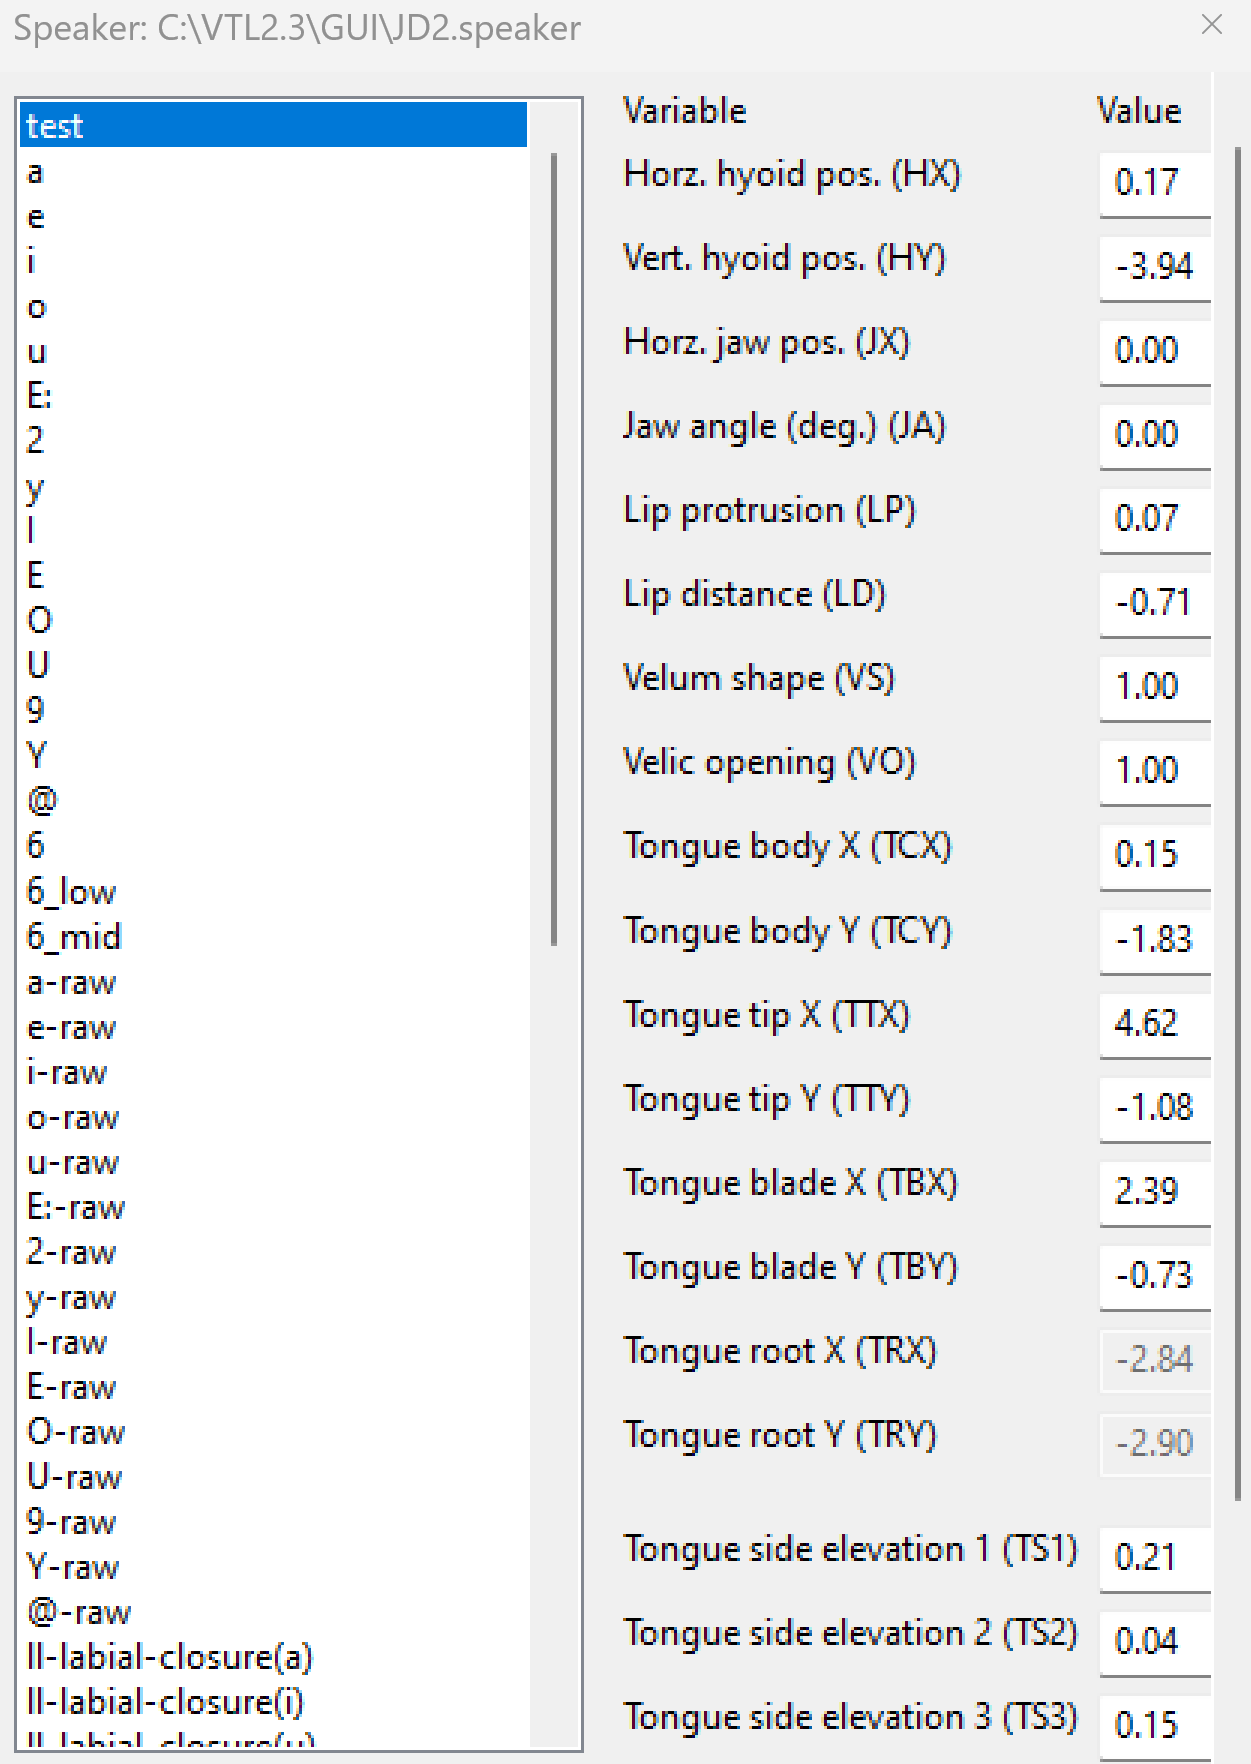
\includegraphics[width=0.6\textwidth]{C:/Users/MJM/OneDrive/桌面/Audio Processing/homework2/pic/SpearkerVariable1.png}
		\caption{The variable of the speaker}
		\label{fig:speaker-variable}
	\end{figure}
	
	\begin{figure}[h!]
		\centering
		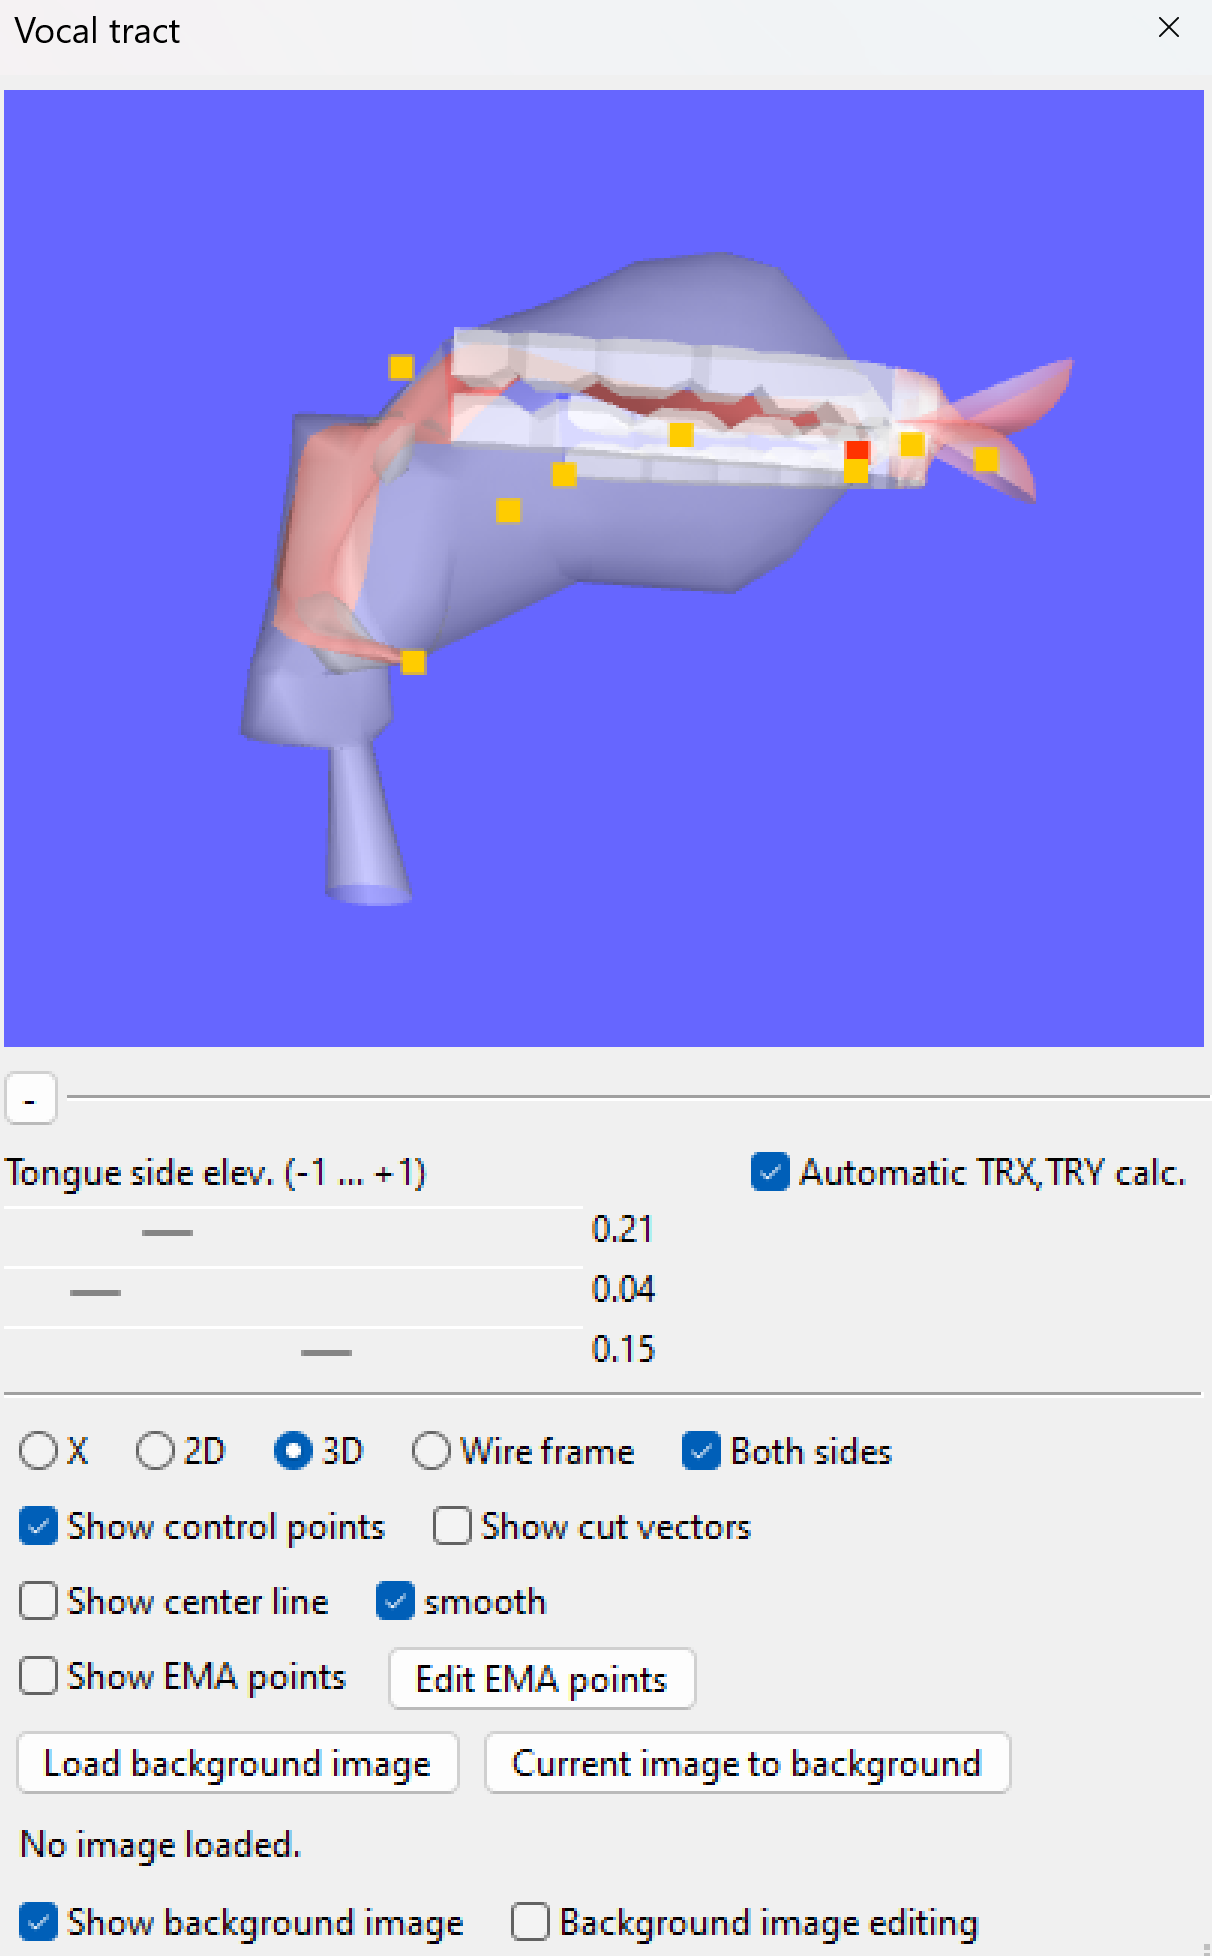
\includegraphics[width=0.6\textwidth]{C:/Users/MJM/OneDrive/桌面/Audio Processing/homework2/pic/vocalTract1.png}
		\caption{The vocal tract shape}
		\label{fig:vocal-tract}
	\end{figure}

	\section*{}
	\textbf{Question2:}This section contains the main content of your document. You can add more sections or subsections as needed.
	\begin{figure}[htbp]
		\begin{minipage}[t]{0.45\linewidth}
			\centering
			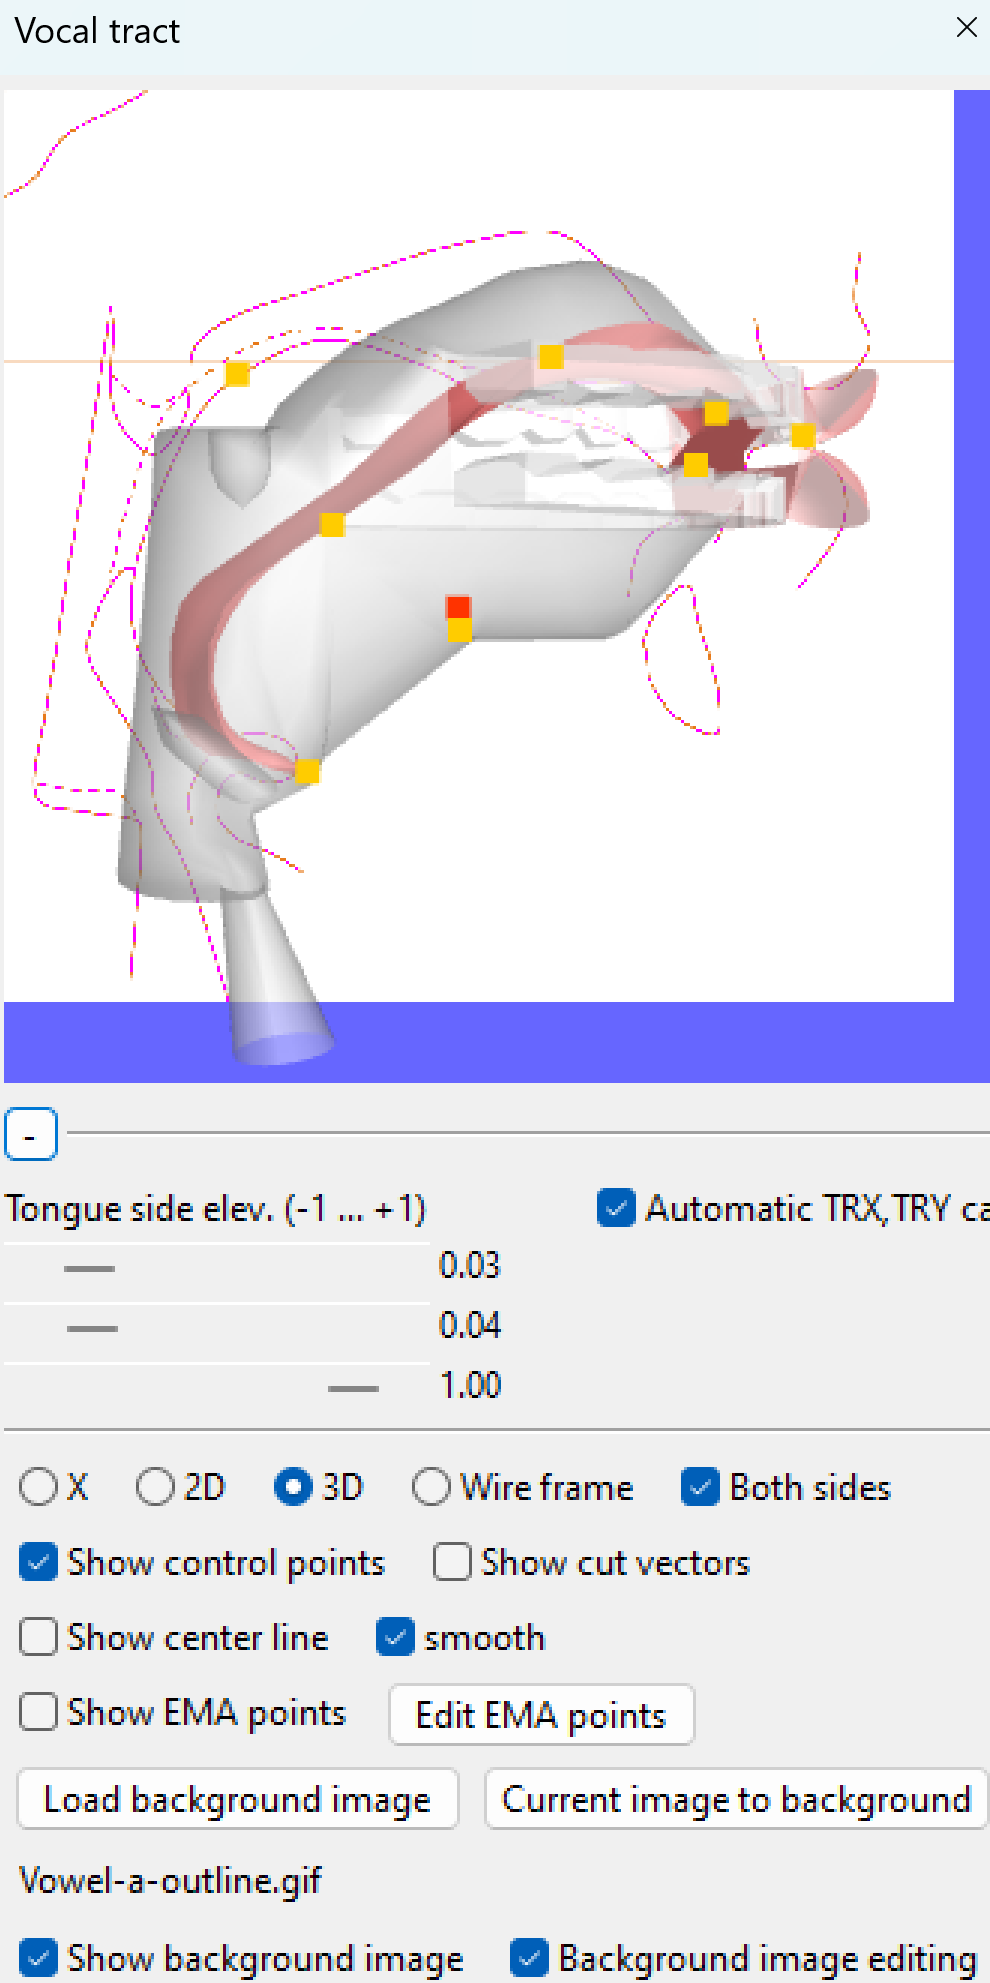
\includegraphics[height=12cm,width=6cm]{C:/Users/MJM/OneDrive/桌面/Audio Processing/homework2/pic/vowel-a.png}
			\caption{vowel-a-3D}
		\end{minipage}%
		\begin{minipage}[t]{0.45\linewidth}
			\centering
			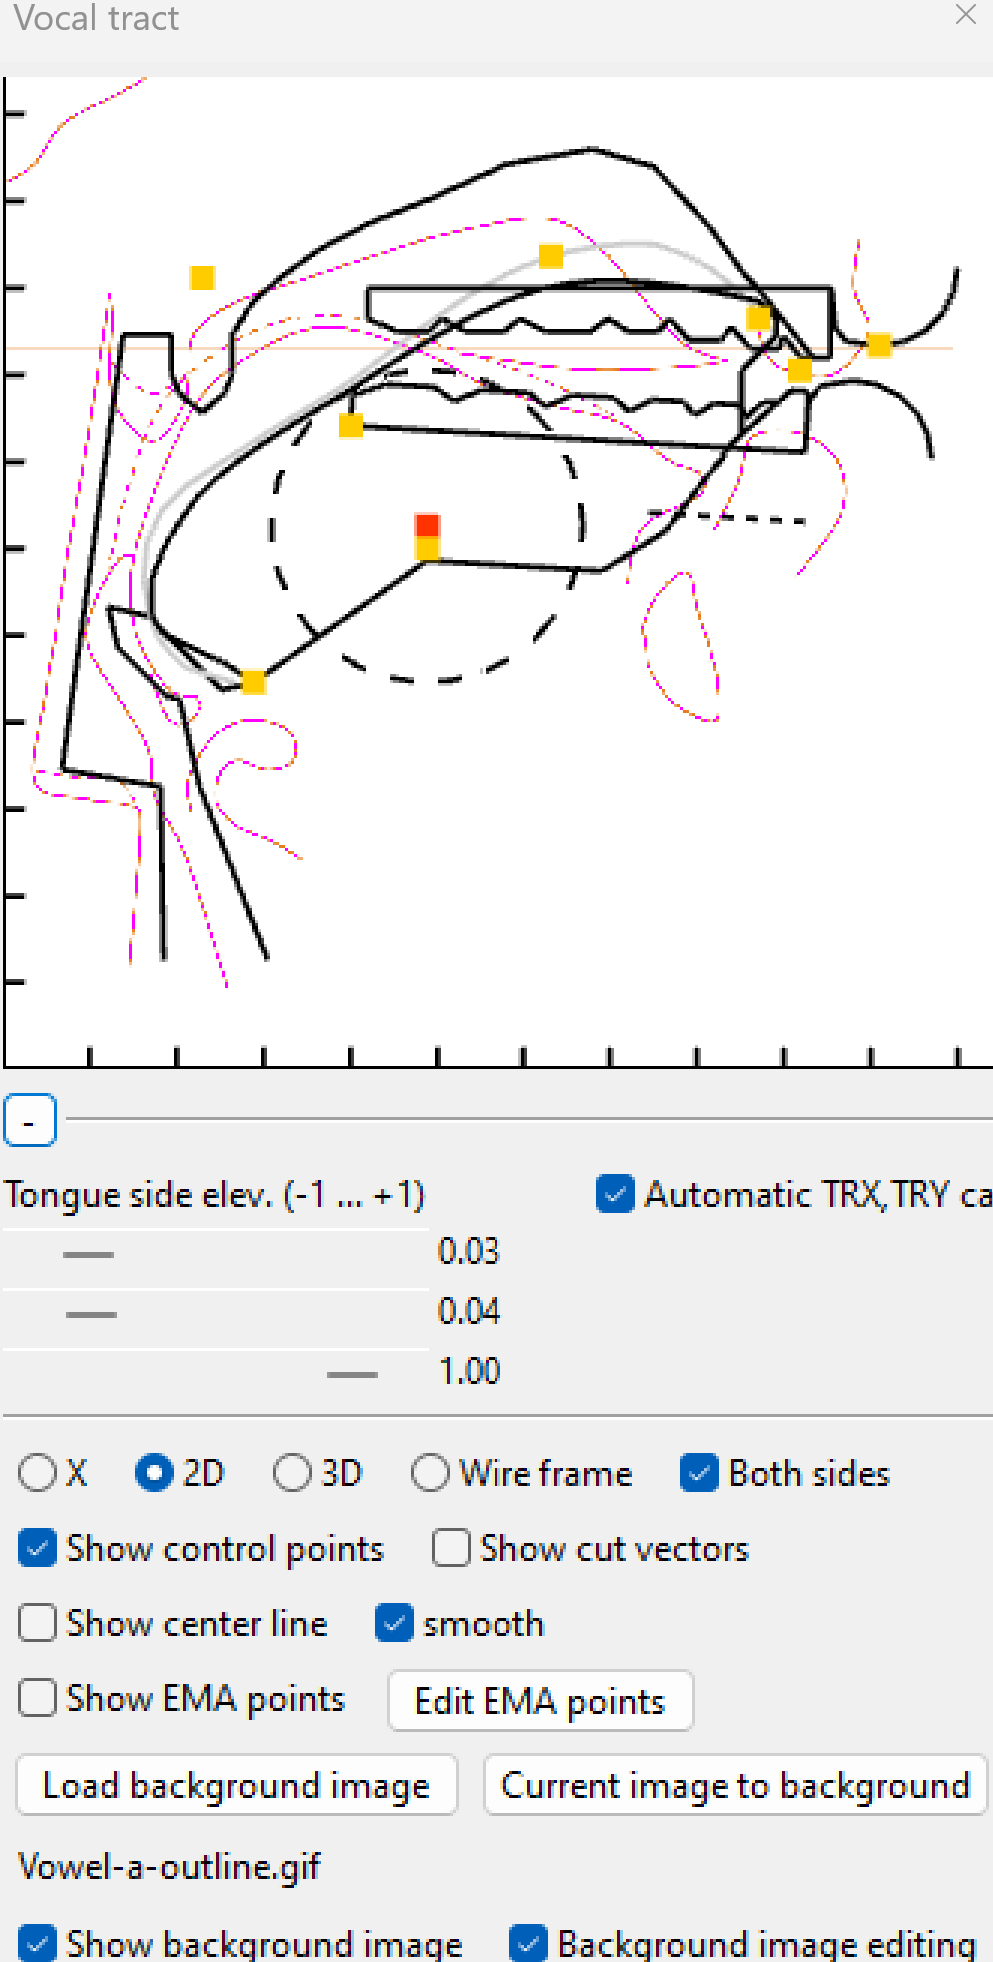
\includegraphics[height=12cm,width=6cm]{C:/Users/MJM/OneDrive/桌面/Audio Processing/homework2/pic/vowel-a-2D.png}
			\caption{vowel-a-2D}
		\end{minipage}
	\end{figure}

	\begin{figure}[htbp]
		\begin{minipage}[t]{0.45\linewidth}
			\centering
			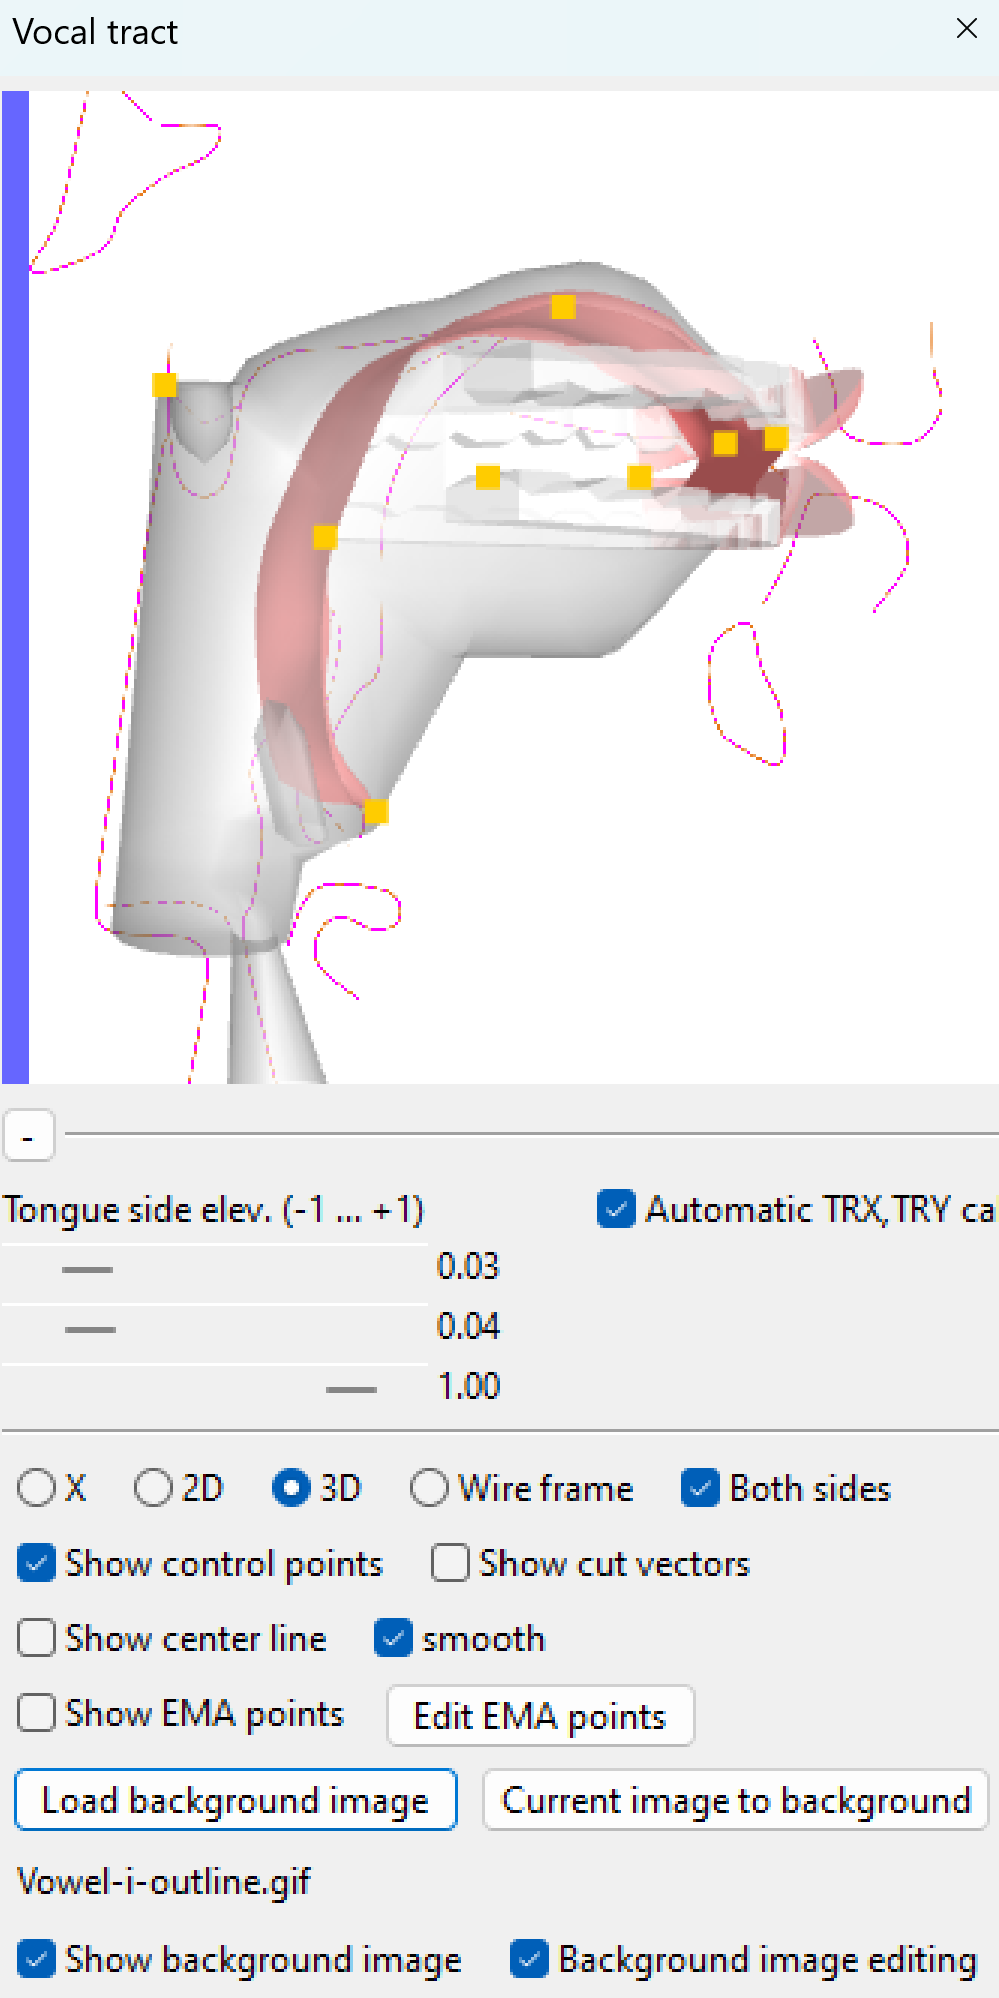
\includegraphics[height=12cm,width=6cm]{C:/Users/MJM/OneDrive/桌面/Audio Processing/homework2/pic/vowel-i.png}
			\caption{vowel-i-3D}
		\end{minipage}%
		\begin{minipage}[t]{0.45\linewidth}
			\centering
			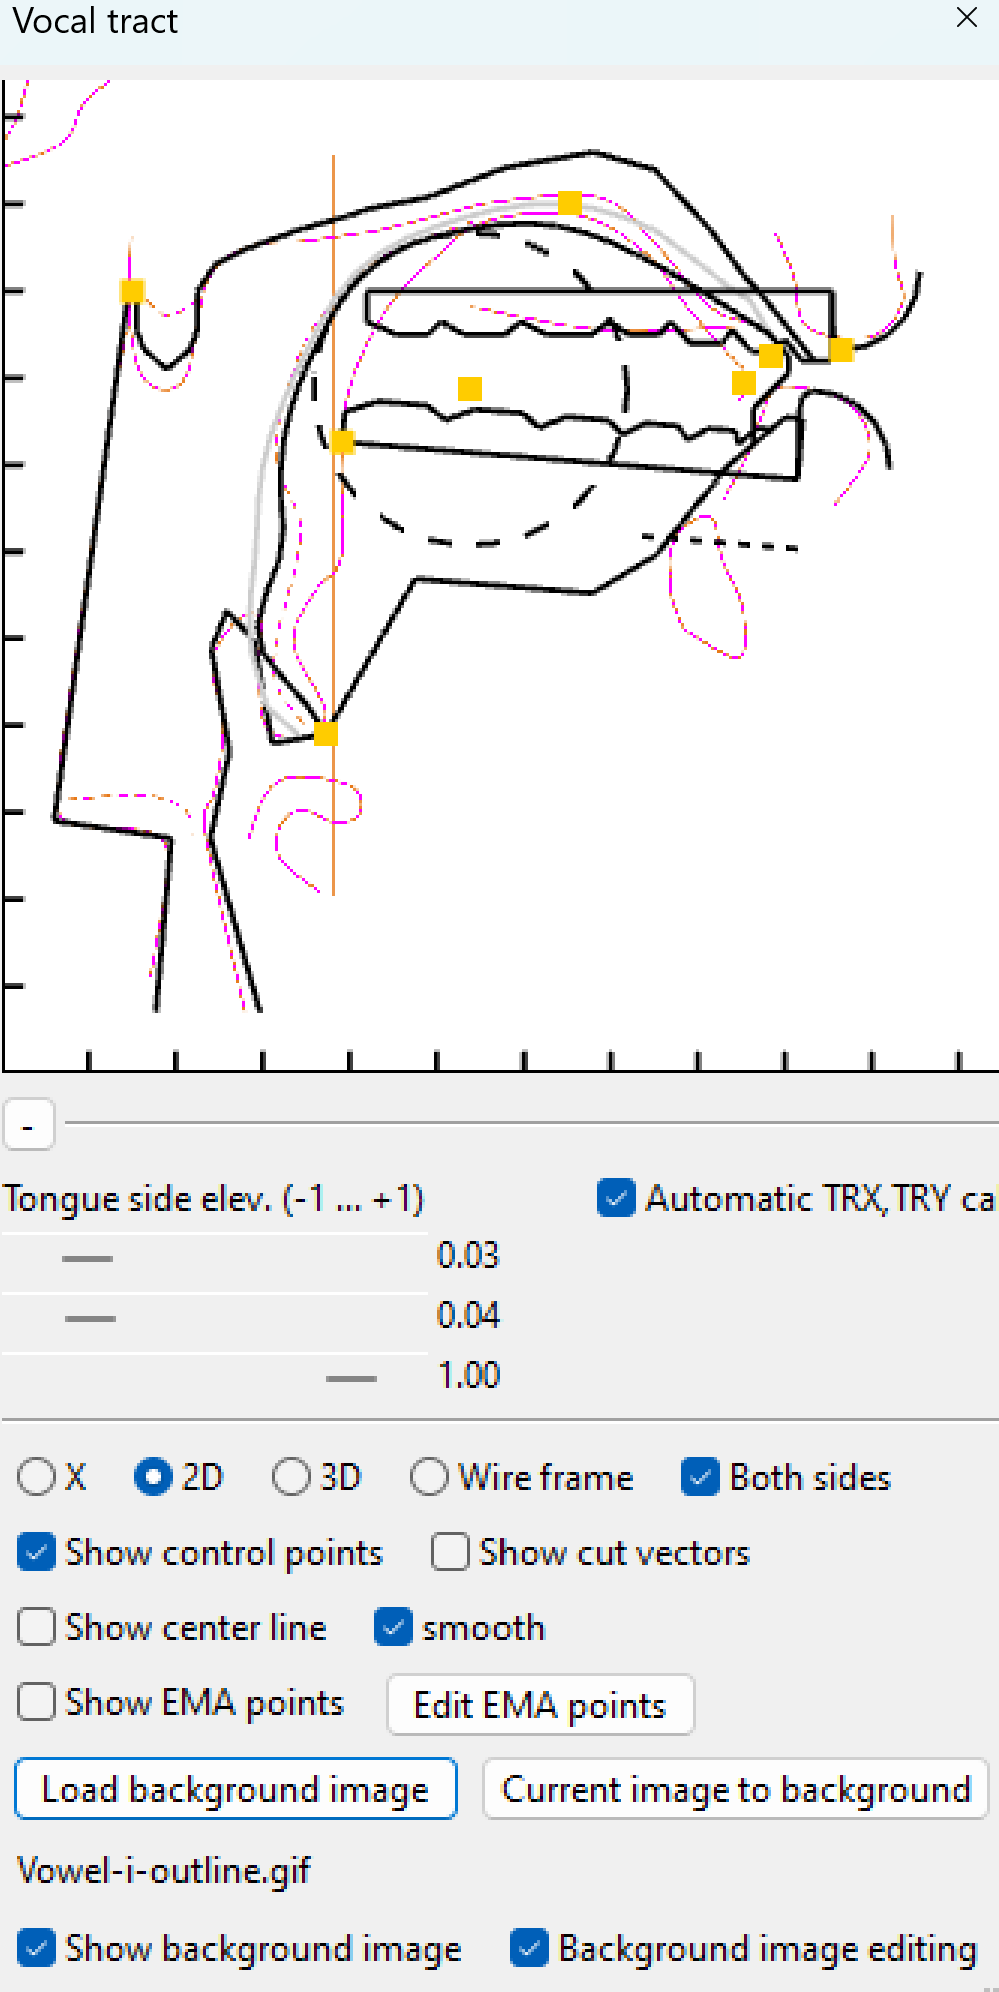
\includegraphics[height=12cm,width=6cm]{C:/Users/MJM/OneDrive/桌面/Audio Processing/homework2/pic/vowel-i-2D.png}
			\caption{vowel-i-2D}
		\end{minipage}
	\end{figure}
	
		\begin{figure}[htbp]
		\begin{minipage}[t]{0.45\linewidth}
			\centering
			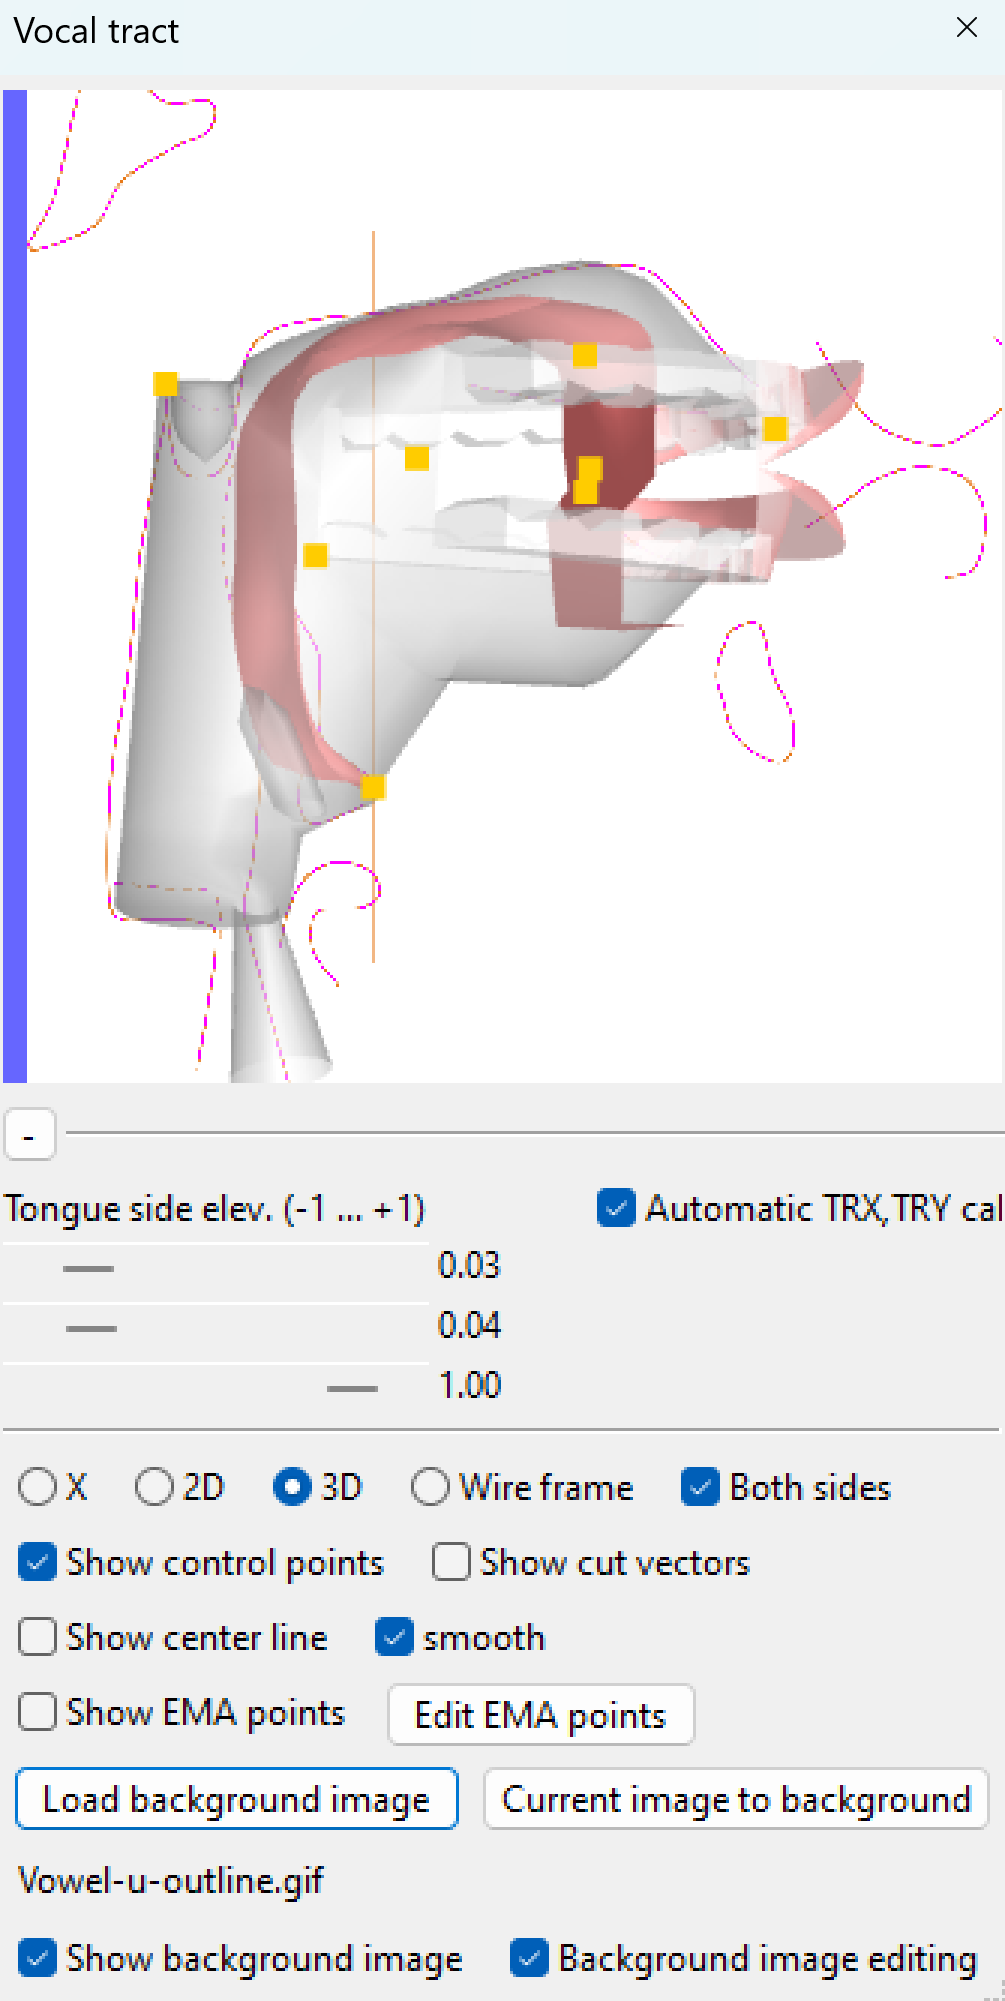
\includegraphics[height=12cm,width=6cm]{C:/Users/MJM/OneDrive/桌面/Audio Processing/homework2/pic/vowel-u.png}
			\caption{vowel-u-3D}
		\end{minipage}%
		\begin{minipage}[t]{0.45\linewidth}
			\centering
			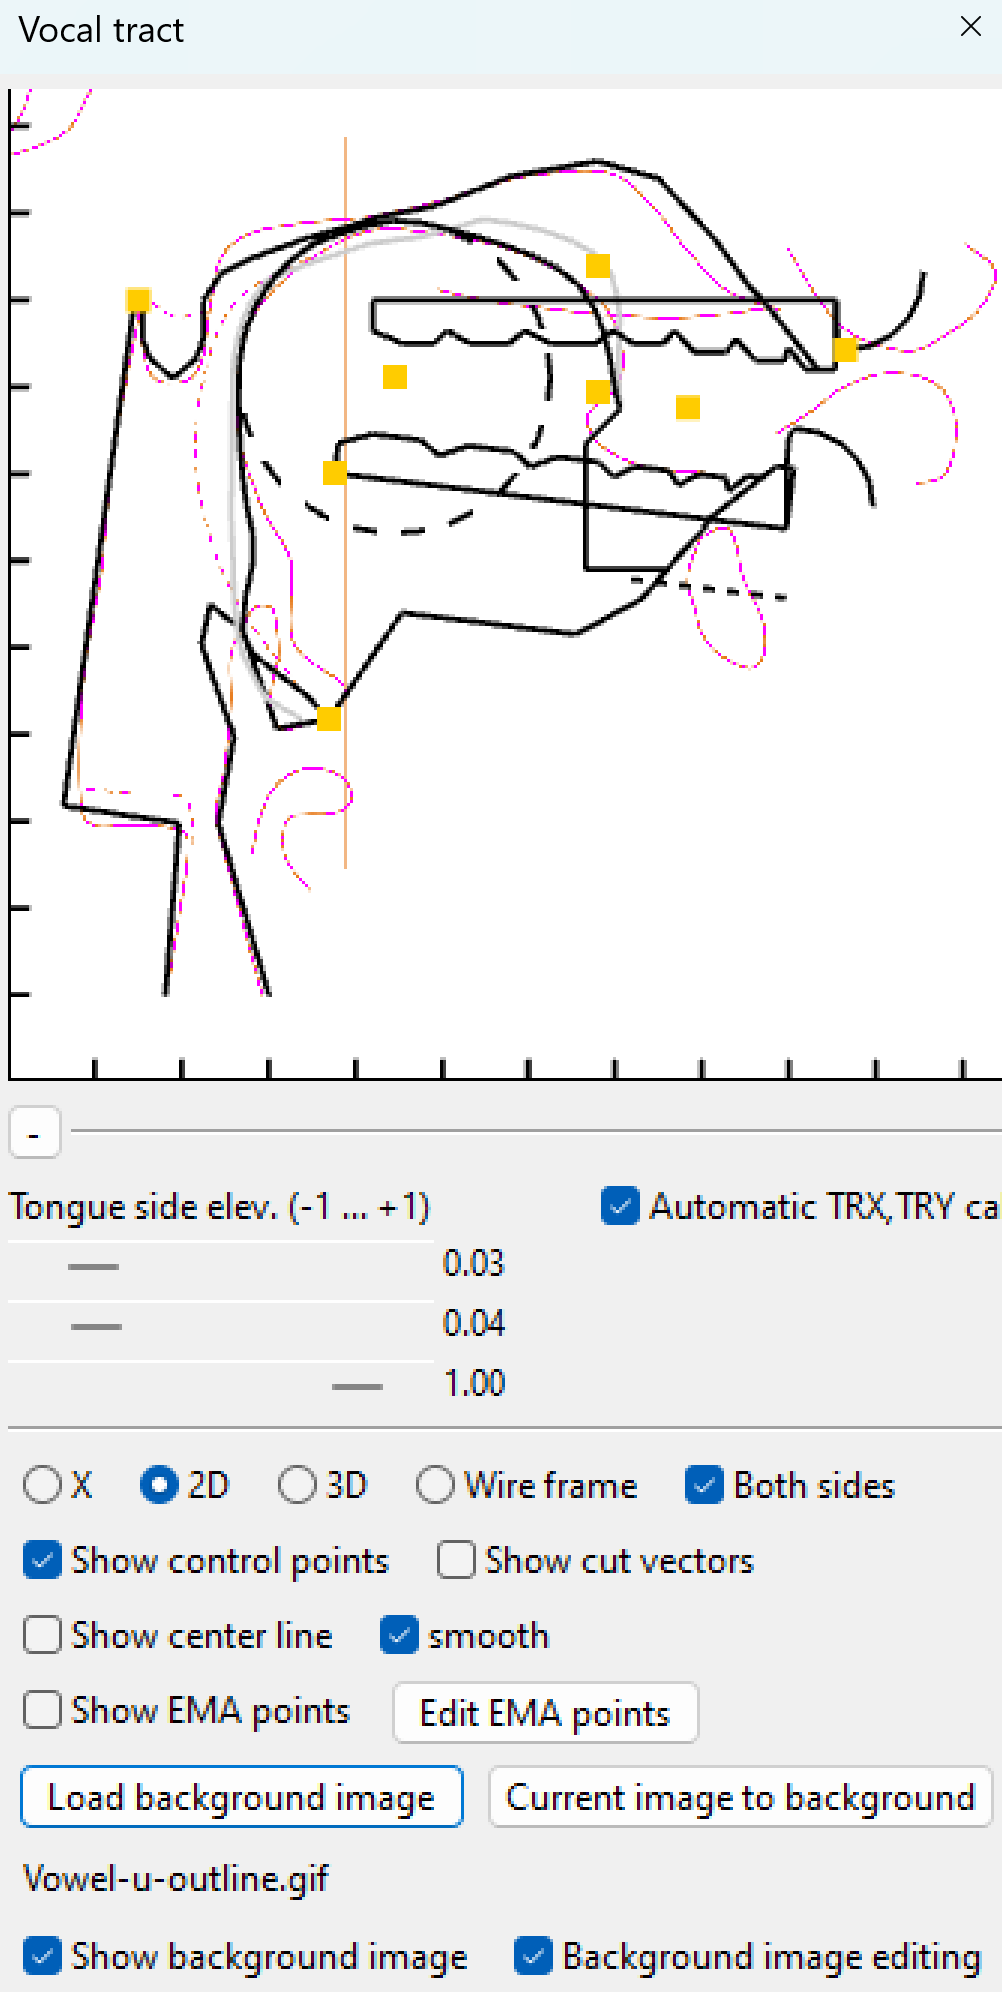
\includegraphics[height=12cm,width=6cm]{C:/Users/MJM/OneDrive/桌面/Audio Processing/homework2/pic/vowel-u-2D.png}
			\caption{vowel-u-2D}
		\end{minipage}
	\end{figure}
	\newpage
	\section*{}
	\textbf{Question3:} I choose example03, change all “modal” glottal shape gestures to “breathy” glottis shapes, change first two tongue tip from alveolar to postalveolar, prolong last tongue tip which alveolar-closure from 235ms to 335ms, and change last vowel gesture from @ to E.
	\begin{figure}[h!]
		\centering
		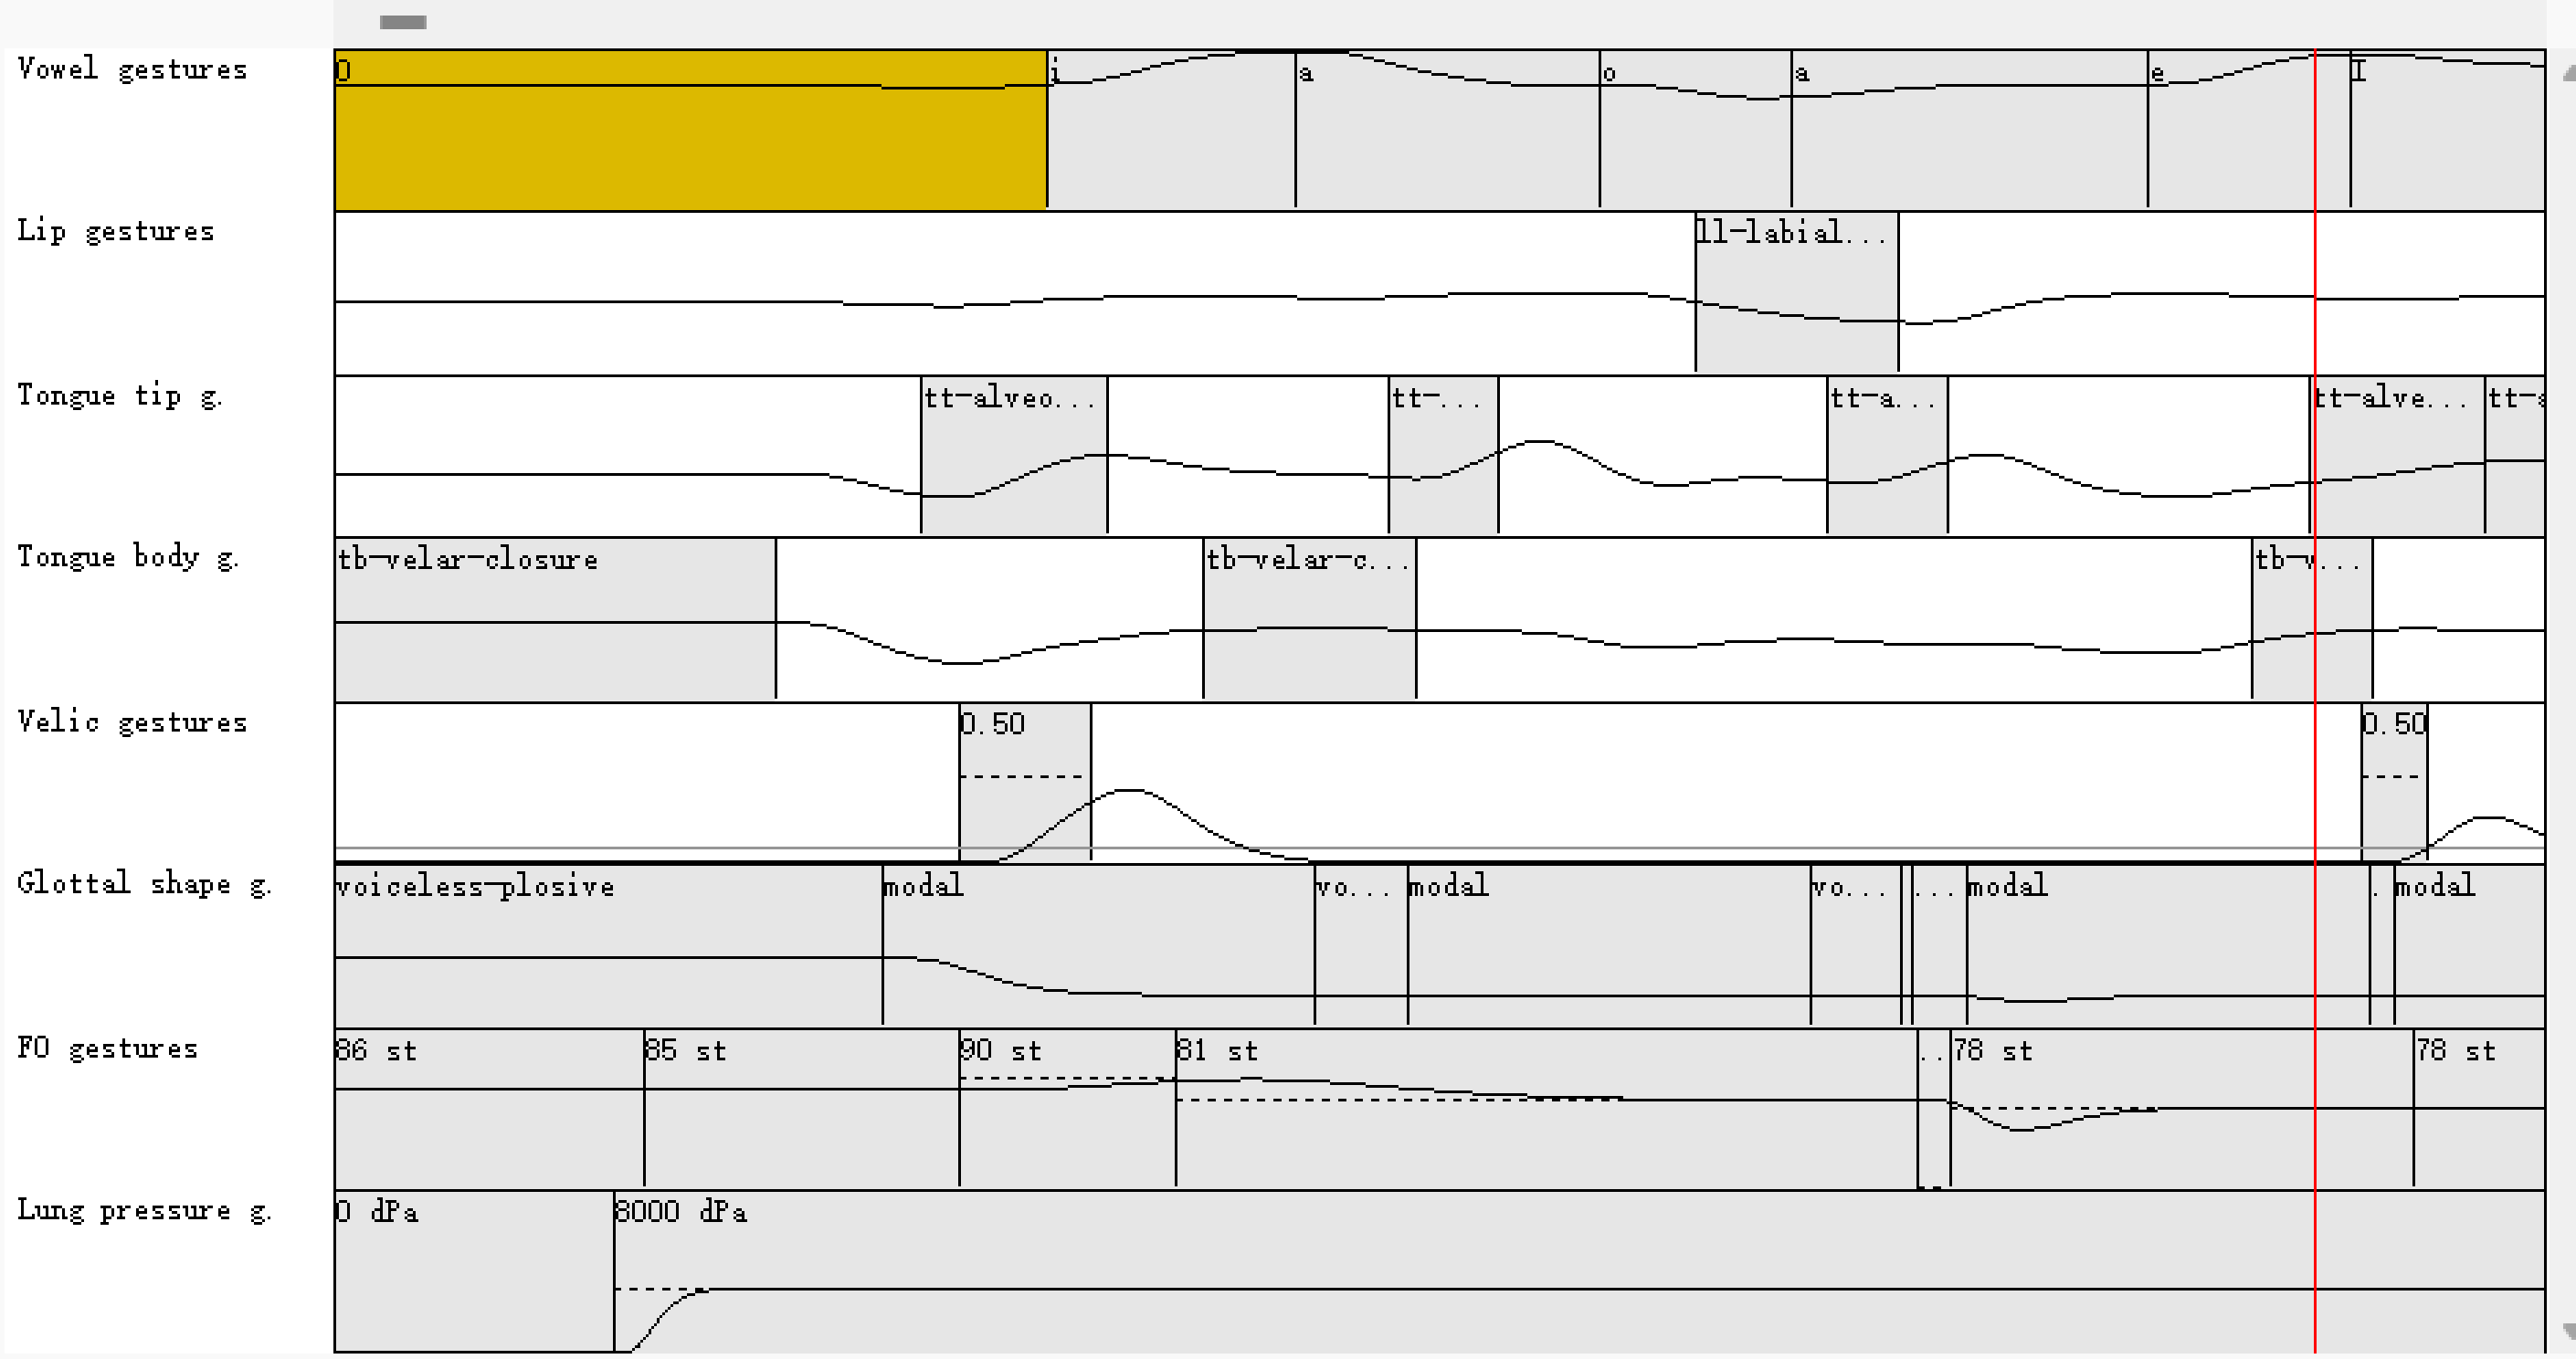
\includegraphics[width=0.8\textwidth]{C:/Users/MJM/OneDrive/桌面/Audio Processing/homework2/pic/original_gesture_score.png}
		\caption{original example}
		\label{fig:original}
	\end{figure}
	\begin{figure}[h!]
		\centering
		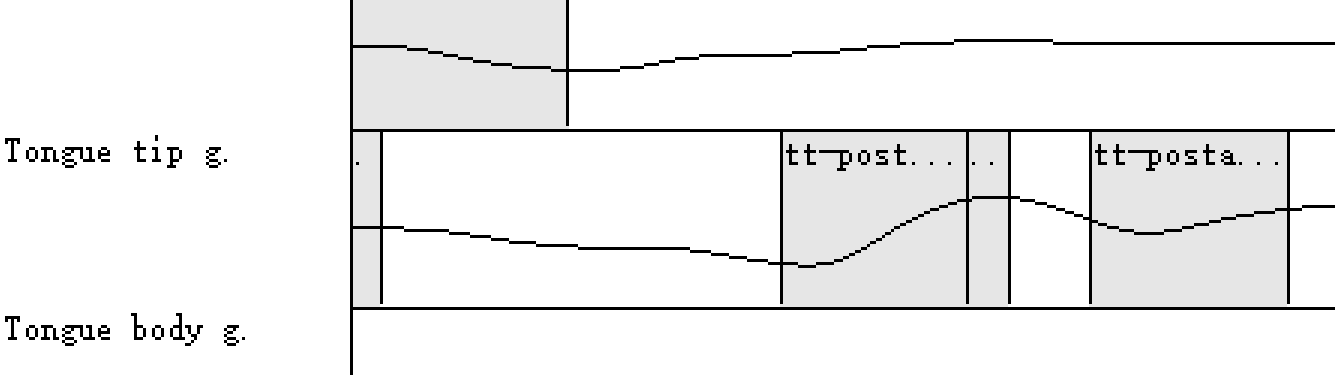
\includegraphics[width=0.8\textwidth]{C:/Users/MJM/OneDrive/桌面/Audio Processing/homework2/pic/tongue-tip-change.png}
		\caption{Tongue tip change}
		\label{fig:tongue tip change}
	\end{figure}
	\begin{figure}[h!]
		\centering
		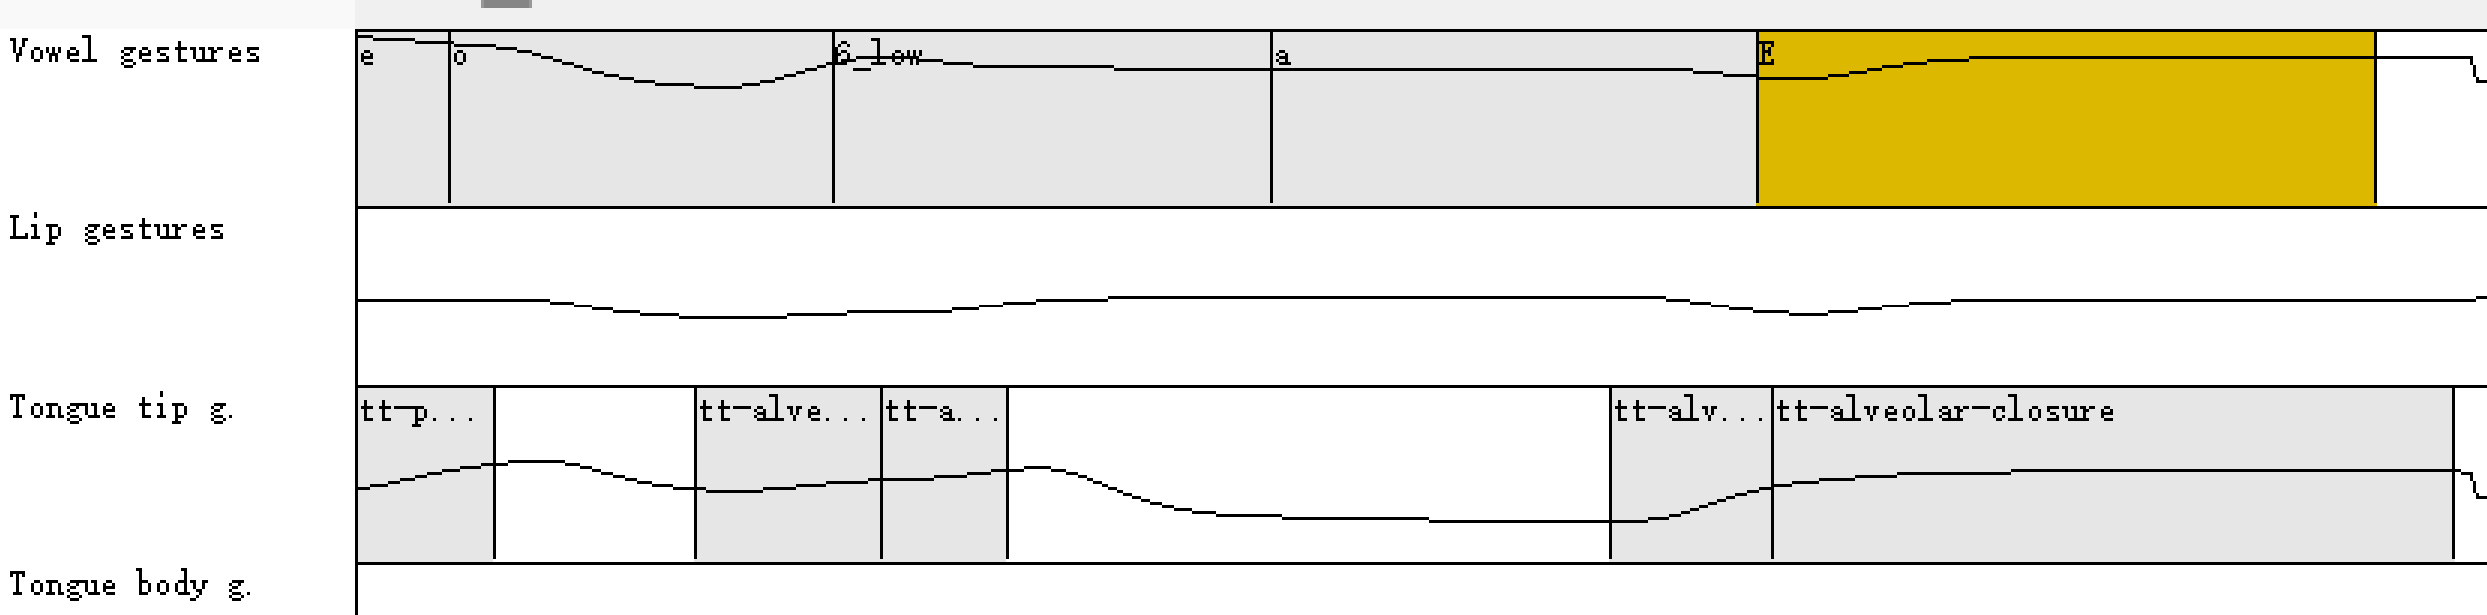
\includegraphics[width=0.8\textwidth]{C:/Users/MJM/OneDrive/桌面/Audio Processing/homework2/pic/last_two_gesture.png}
		\caption{last tongue tip change}
		\label{fig:last two}
	\end{figure}
	\begin{figure}[h!]
		\centering
		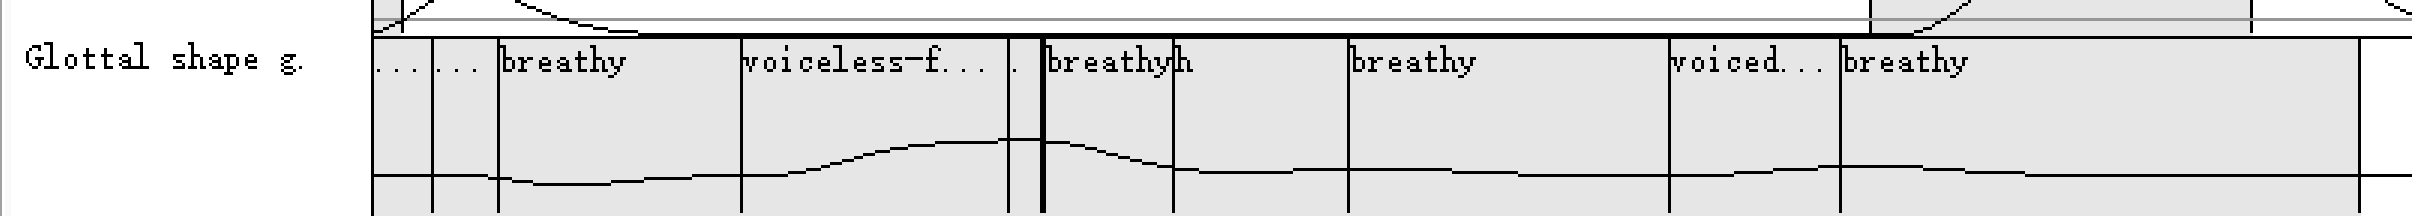
\includegraphics[width=0.8\textwidth]{C:/Users/MJM/OneDrive/桌面/Audio Processing/homework2/pic/glottal_change.png}
		\caption{glottal shape change}
		\label{fig:glottal shape change}
	\end{figure}
		\begin{figure}[h!]
		\centering
		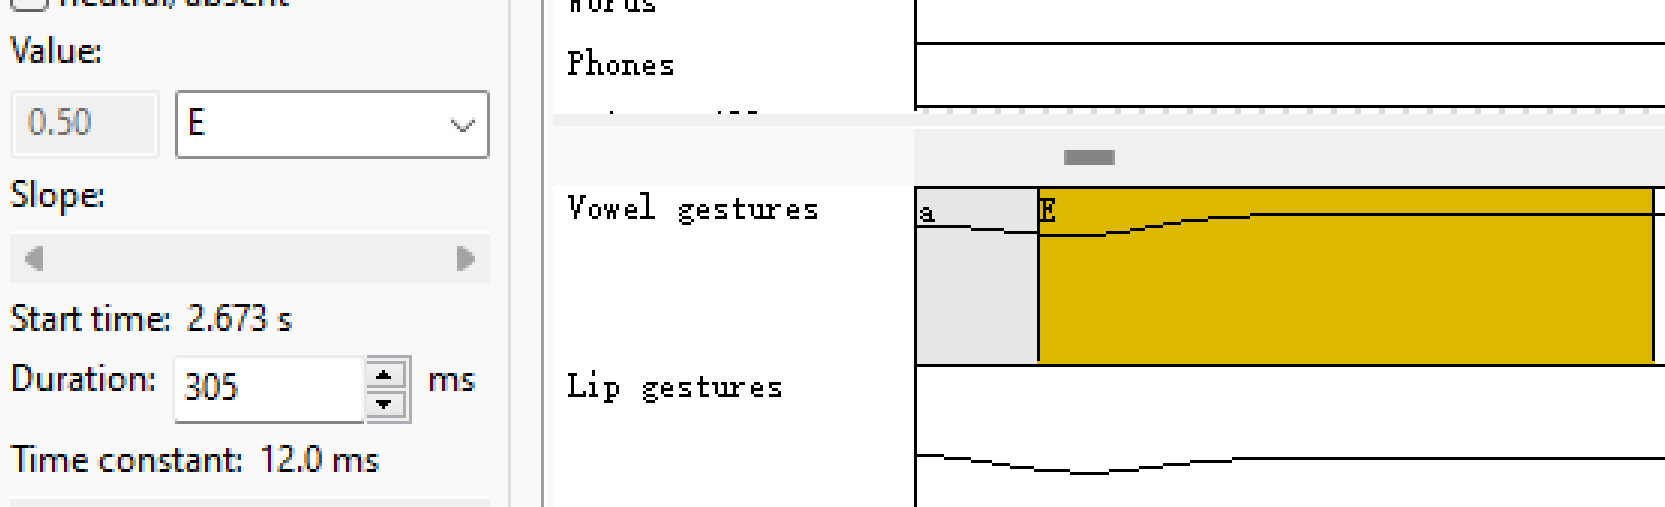
\includegraphics[width=0.8\textwidth]{C:/Users/MJM/OneDrive/桌面/Audio Processing/homework2/pic/vowel_value_change.png}
		\caption{vowel value change}
		\label{fig:vowel value change}
	\end{figure}
	\section*{}
	\textbf{Question4:}I made "I will owe you eight."
	This includes five vowel words: "I," "will," "owe," "you," and "eight."
	
\end{document}
